Effective management of facilities is a key challenge in the healthcare domain
 to reduce costs and procedure times and improve the overall quality of services for both the patients and medical staff. 
%
In this context, operating rooms are considered one of the most critical and expensive resources in a hospital environment, due to their high operational costs, the complexity and relevance of the surgeries that take place within them.

Surgery schedules and allocation of operating rooms and medical teams are now usually managed through manual processes that rely on the accumulated expertise of the medical staff. 
% 
Given the ever-increasing digitalization trend in healthcare, the next generation of hospital information systems should allow for better overall management and monitoring of such facilities, to support the medical staff in the planning and allocation of resources.


The typical complex task in the context of Operating Room Management (ORM) is strictly related to the identification of optimized planning of surgery schedule that prioritizes surgeries and maximizes the utilization of resources while minimizing waste of time and poor exploitation of resources.
%
Generally speaking, the system running around the (peri-)operative context can be seen as an ecosystem of surgeons, nurses and anesthesia health care providers, who must smoothly coordinate their work to deliver high-quality surgical care.
%
Moreover, limited physical resources that are exploited in the process---the operating room itself and its supporting systems, but also specific biomedical equipment---are part of the ecosystem and must be considered when planning the surgery schedule.

The timely execution of the surgical workflow might be influenced by:
\begin{itemize}
\item the composition of the team and the interactions between different professional figures;
\item the availability of the required equipment and facilities;
\item the specific characteristics of the patient and the surgery to be performed;
\item the potential for unexpected events or complications during surgery;
\item the risk of surgery cancellation.
\end{itemize}
%
Planning surgeries means considering all these (and more) factors to provide the best possible service.
%
In the current practice, ORM often relies on the experience and intuition of staff, which can lead to suboptimal performance in operating theaters, as it is challenging to account for all requirements from the various stakeholders involved.

The literature offers a range of methods primarily grounded in mathematical and computational models to support and enhance ORM.
%
These approaches enable more accurate perioperative risk assessments and optimized resource allocation~\cite{Zhu2019}.
%
A prominent example is the use of Artificial Intelligence, particularly Machine Learning, which leverages large datasets from operating suites to develop predictive models.
%
These models can forecast factors such as surgical case duration, risk of cancellation, and post-anesthesia care unit occupancy, thereby facilitating the creation of safer and more efficient surgery schedules~\cite{Fairley2019, luo2020hij}.
%
Other AI-based strategies include the integration of multi-objective optimization models with metaheuristic techniques, as demonstrated in~\cite{aringhieri2022eor} for surgery scheduling, and the use of hybrid genetic optimization models, as proposed in~\cite{GUIDO2017}.
%
Simulation-based approaches are also explored in the literature.
%
For instance,~\cite{Schoenfelder2021} presents a flow-chart-based model of the operating room workflow, which is used to simulate scenarios and evaluate management policies according to indicators such as patient waiting time, idle time, and the number of postponed surgeries.

All these factors make adopting a \ac{DT}-based approach particularly suiting for ORM.
%
\acp{DT} can support the automatic collection of data concerning operating room planning and utilization and construct models that can be used to evaluate new policies, hence supporting the future allocation of resources.

%=======================================================
\section{Case Study Analysis}
%=======================================================



Managing ORM effectively is a crucial goal for \ausl{}. 
This is a complex task due to the large number of operating rooms (more than 90) distributed across 10 different hospital facilities, each with its own peculiarities in the management of the surgery process.
%
Currently, planning is mainly performed manually with a meeting of the surgical board of each hospital on a weekly basis.
%
Operating rooms slots (typically half-day periods) are assigned to different surgical specialties, which may fit how many surgeries per-slot depending on their expected duration. 

Tracking of the actual execution of surgeries, is partially automated and relies on a QR code scanning system, a printed schedule of the planned surgeries for the day and a paper form for each surgery that is filled by hand by the medical staff.

The QR scanning system is designed to allow keeping track of the most relevant phases of a surgical procedure.
Additional steps might be possible, depending on the facilities available (e.g. dedicated induction rooms for anesthesia, recovery rooms, etc.), but the main phases that are always present in every surgery are the following:

\begin{enumerate}
    \item Patient exits the hospital ward
    \item Patient enters the operating suite
    \item Patient enters the operating room\footnote{From now on if, for any unexpected reason, the surgical procedure is interrupted step 8 is the next one}  %% questo credo possa avvenire prima di Anesthesia performed, in generale. Esistono casi per i quali l'anestesia inizia fuori dalla sala operatoria, ma dipende dalla disponibilità o meno, nel blocco, di aree dedicate
    \item Anesthesia is performed\footnote{In some cases this step can happen before step 3 if there are dedicated facilities to support it}
    \item Anesthesia is effective
    \item Surgery is started
    \item Surgery is completed
    \item Patient is moved outside the operating room
    \item Patient leaves the operating suite
    \item Patient enters a hospital ward (which can be different from the one which he came from)
\end{enumerate}
%
After a surgical procedure, the operating room is cleaned and prepared for the next one.
This process involved the sterilization of the room and reusable equipment, as well as the disposal of any medical waste produced during the surgery.

Timing of each step execution is also annotated on the paper form,
one of the main current issues is the discrepancy between the time the QR codes are scanned and the time steps are actually performed, as there might be a delay in reporting or scanning resulting in inaccurate data.
%
This is due to the fact that the medical staff is usually very busy and focused on the patient and can forget to scan at the appropriate time.
The paper form allows them to correct the timings annotating afterwards making an estimate of what they remember doing as well as other relevant information about the surgery, which they may find useful to keep track of.
%
This process is also supported by a Surgical-Safety CheckList (SSCL) that ensures that protocols are followed to enhance patient safety and reduce risks of errors during surgery.
%
The checklist covers patient admission, pre-surgery, and post-surgery phases, forcing the medical staff to verify critical information at each step. 


Another critical issue with the current state of the system is that data registered by the QR scanning system is stored in a database that is local to each hospital. This, of course, implies that the coordinators that need to manage the network of operating rooms are not able to automatically retrieve information about the current state of the ongoing surgical procedures, leading to less efficient management.

The main pain points that emerged in the conversation with the medical staff are here summarized:
\begin{itemize}
    \item Low readability of manually annotated data
    \item Limited space on the paper form to annotate surgery's steps
    \item Discrepancy between the scanned times and the real times
    \item Deletion or delay of planned surgery is currently not tracked since the schedule is printed
    \item Accountability for issues regarding data collection is impossible to define
    \item Sub-optimal management of operating rooms due to the fact that the availability of a facility is not known in real-time
\end{itemize}

From the analysis of the current situation and the staff needs the following functional requirements for a new management system are defined:
\begin{itemize}
    \item Real-time monitoring of the availability of operating rooms: whether they are busy at the moment and what the planned surgeries for each one are
    \item Time monitoring of surgical procedures and individual procedures' steps to understand the overall efficiency
    \item Automatic generation of warnings when there is inconsistency in the transmitted data (e.g. two patients in the same room at the same time, a step that is taking an unexpected amount of time)
    \item Storage of detected warnings for historical data analysis
    \item Easy data access through a dashboard to visualize the current state, review warnings, and annotate steps. The dashboard should also be accessed through an account to solve the problem of accountability.
\end{itemize}

From a more technical point of view, the new system is also required to be integrated with the existing solution, and to support interoperability with other future possible systems that may require access to data.

%=======================================================
\section{\acl{DTE} Proposal}
%=======================================================

In this section, we provide a description of a \acp{DTE} designed to collect data and monitor ongoing surgeries to support ORM.
%
Assuming to adopt DTs as a pervasive approach, we can envision having an ecosystem of connected DTs that can map real-world facilities.
%
Each hospital can have its own DT, connected to DTs of each operating roomwhich can be connected to those of the medical equipment available in each room.
%
Similarly, we can mirror people, namely patients and the medical staff, to track their interactions with facilities and each other.

\begin{figure}
    \centering
    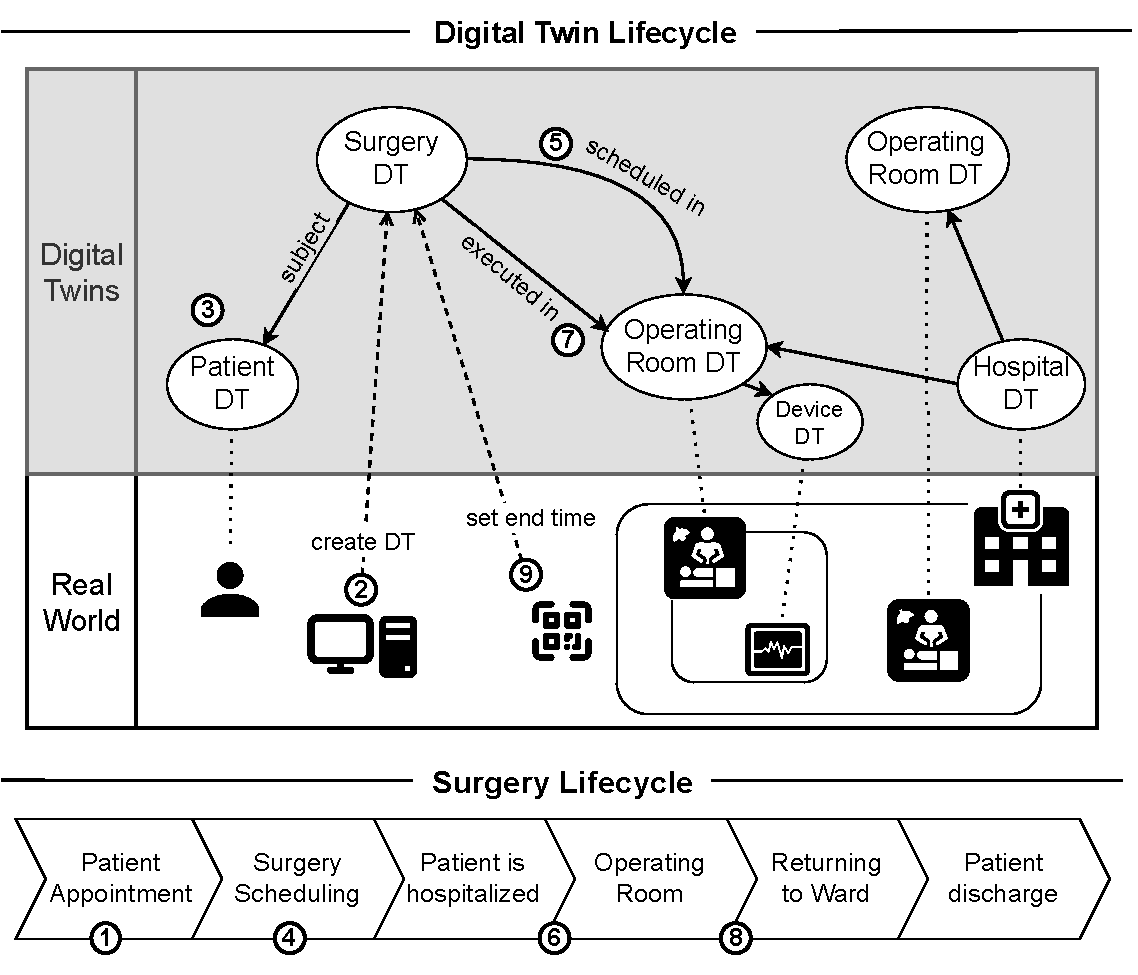
\includegraphics[width=\columnwidth]{figures/orm/DTORM.pdf}
    \caption{An example of how a DT ecosystem could support the management of ORs as well as the real-time tracking of elective surgery processes.}
    \label{fig:dt-orm-ecosystem}
\end{figure}

The resulting \ac{DTE} can represent the state of the operating rooms at any given time, \Cref{fig:dt-orm-ecosystem} shows an overview of the planned \ac{DTE} architecture, and its relationship with the surgical process.
%
When a doctor and a patient meet for an appointment and the need for a surgical procedure is identified \circled{1} a new \textit{Surgery DT} is created \circled{2} and linked to the \emph{Patient DT} \circled{3}. 
%
Then, whenever the surgery is scheduled in a specific room \circled{4} a relationship with the \emph{Operating Room DT} is added to keep track of the planned surgeries per each room \circled{5}.
%
The patient is then usually hospitalized and transferred to the operating room \circled{6}. When the patient actually enters the room the \textit{Surgery DT} creates a new relationship with the \emph{Operating Room DT}\footnote{For any reason it could also be a different room from the planned one.} \circled{7} which will report that the room is busy.
%
Finally, when the patient leaves the room \circled{8}, the end time is registered---e.g. by scanning a barcode like in our case study---\circled{9} and the operating room can now be set back to an available state after the necessary cleaning operations.


The main responsibilities of the identified \acp{DT} in the context of ORM are summarized in \Cref{tab:dt-responsibilities}.

\begin{table}
\centering
\small
\begin{tabularx}{\textwidth}{|p{3cm}|X|}
\hline
\textbf{DT Type} & \textbf{Responsibilities} \\
\hline
Patient DT & Stores all patient-related data, including personal and historical data. Mostly static, but forms relationships with other DTs during the surgical process. If indoor localization is possible, tracks the patient's real-time position. \\
\hline
Surgery DT & Tracks different stages of the surgical process and associated measured times. Relationships allow understanding of the surgery in the context of team, patient, and equipment. Before surgery, estimates time and expresses requirements; during surgery, reflects real-time state and emits warnings on unexpected durations; after surgery, serves as a source for planning and patient history. \\
\hline
Operating Room DT & Tracks the state of the room and its equipment, showing real-time and planned availability. Emits warnings if equipment is damaged or cleaning is necessary. \\
\hline
Vital Monitor DT & Medical IoT device recording patient data during (and potentially before/after) surgery. Shares data with the Patient DT for historical records, possibly via dynamic DT composition. \\
\hline
Hospital DT & Aggregates information about operating rooms and provides a general summary of availability. May encapsulate scheduling and planning for associating operating rooms to surgeries. \\
\hline
Medical Staff DT & Represents a staff member, tracking job scheduling, shifts, vacations, roles, and qualifications. Serves as a data source for scheduling. \\
\hline
Stocks DT & Monitors medical devices and consumable resources stocks and can signal or automatically generate supply orders when thresholds are reached. Warns if stocks are expiring to enable relocation. \\
\hline
\end{tabularx}
\caption{Main responsibilities of the identified DTs in the context of ORM.}
\label{tab:dt-responsibilities}
\end{table}


%=======================================================
\section{Implemented Solution}
%=======================================================

A prototype \ac{DTE} has been implemented to demonstrate potential benefits introduced by the proposed approach in the context of ORM.
%
The prototype focuses on the real-time monitoring of ongoing surgeries, and the ability to verify the consistency of data reported by the automatic scanning system, allowing the medical staff to be notified of anomalies and supporting the amendment of incorrect data. 

\begin{figure}
    \centering
    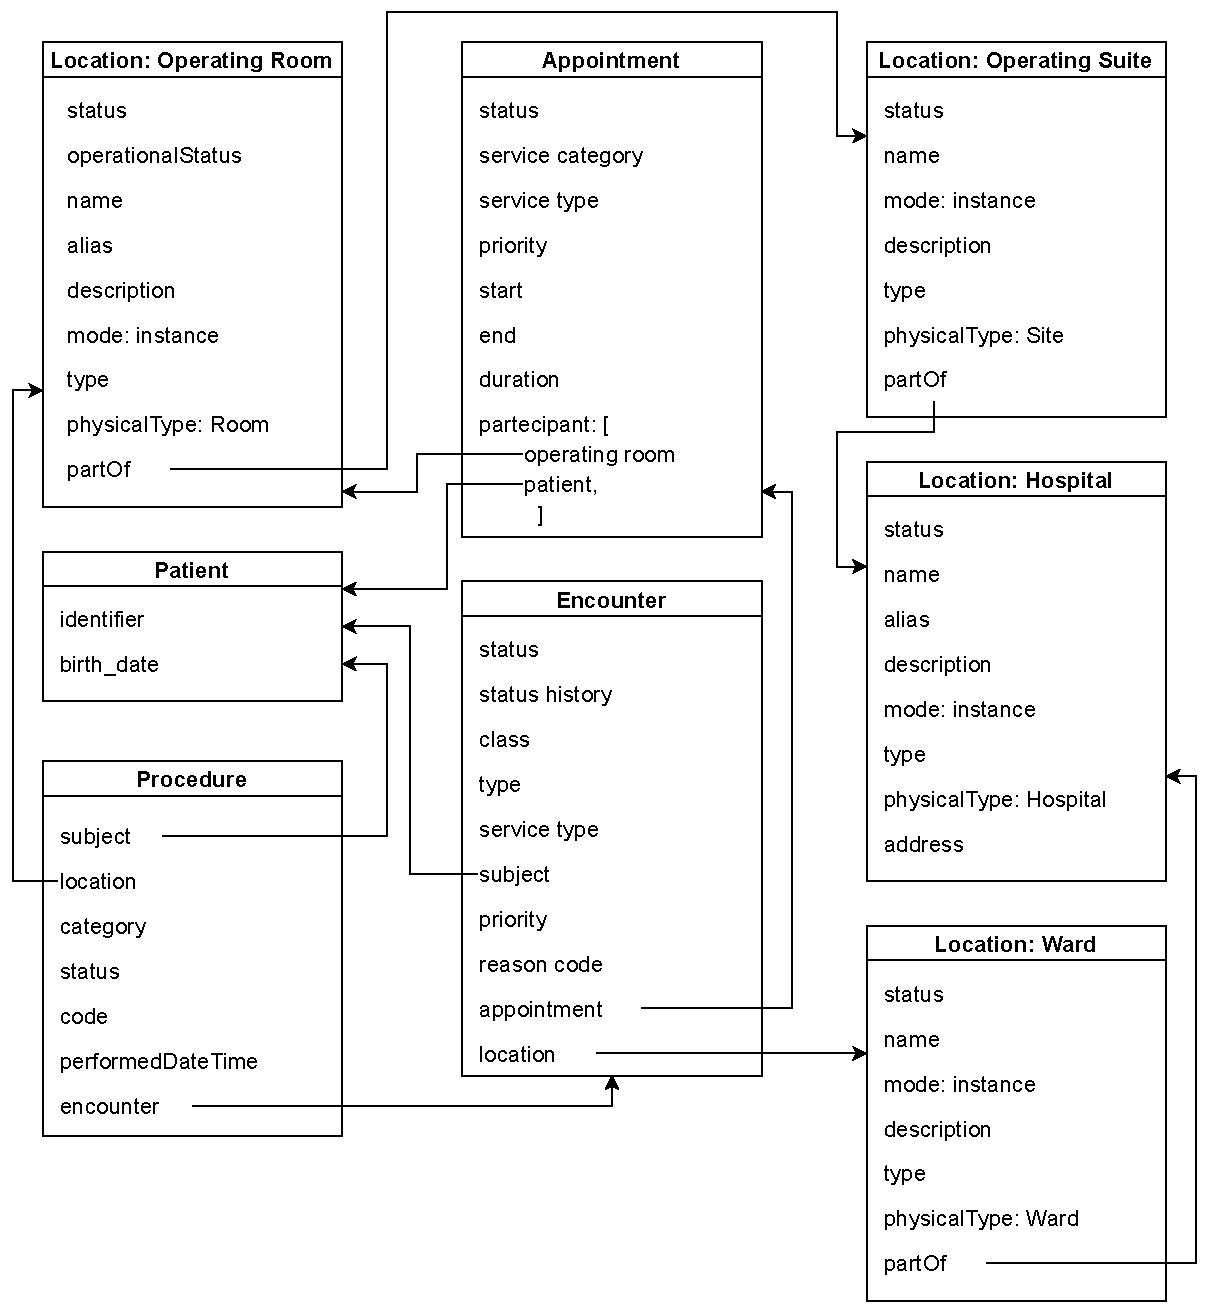
\includegraphics[width=\textwidth]{figures/orm/FHIR_mapping.pdf}
    \caption{The final FHIR resources mapping data related to operating rooms and procedures.}
    \label{fig:orm:fhir_mapping}
\end{figure}

Entities in the domain have been modeled in FHIR for standard healthcare data representation as shown in \Cref{fig:orm:fhir_mapping}.
%
The \ac{DT} layer is used to to translate the existing data sources into FHIR resources, promoting interoperability and standardization.
%
The main resources that the system needs to manage are the various \textit{locations}---namely the hospital structure, the operating suite, the wards and the operating rooms---the \textit{patient} and the surgery which has been mapped in three different connected FHIR resources which are
\begin{itemize} 
    \item the \textit{appointment} defining the nature of the planned surgery, its expected duration and its priority
    \item the \textit{encounter} which is a generic resource for whenever patients and medical staff interact 
    \item and multiple individual \textit{procedure}s which represent each action performed on the patient during the overall surgery process and are linked to the same encounter.
\end{itemize}

The Surgery \ac{DT} supports a basic anomaly detection algorithm that verifies the consistency of the data being reported by the scanning system and can produce warnings in case data is missing or is not coherent with the expected behavior (e.g., surgery is excessively long compared to the expected duration, surgeries overlap in the same room).
%
The Operating Room \ac{DT} maintains the state of the room (available or busy) and the list of planned surgeries for that room.

Finally, a prototype management dashboard is implemented as a web application using the \acp{DT} as the source of data.
%
The dashboard displays the list of all operating rooms, showing their current state and planned surgeries, as shown in \Cref{fig:orm:surgical_procedures_dashboard}.
%
Additionally, for each surgery it is possible to expand the view and resolve any warning generated by the anomaly detection algorithm, as well as to visualize and annotate each step of the surgical procedure.
%
Annotations and edits are stored alongside which user made them, solving the accountability issue present in the current system. 

\begin{figure}
    \centering
    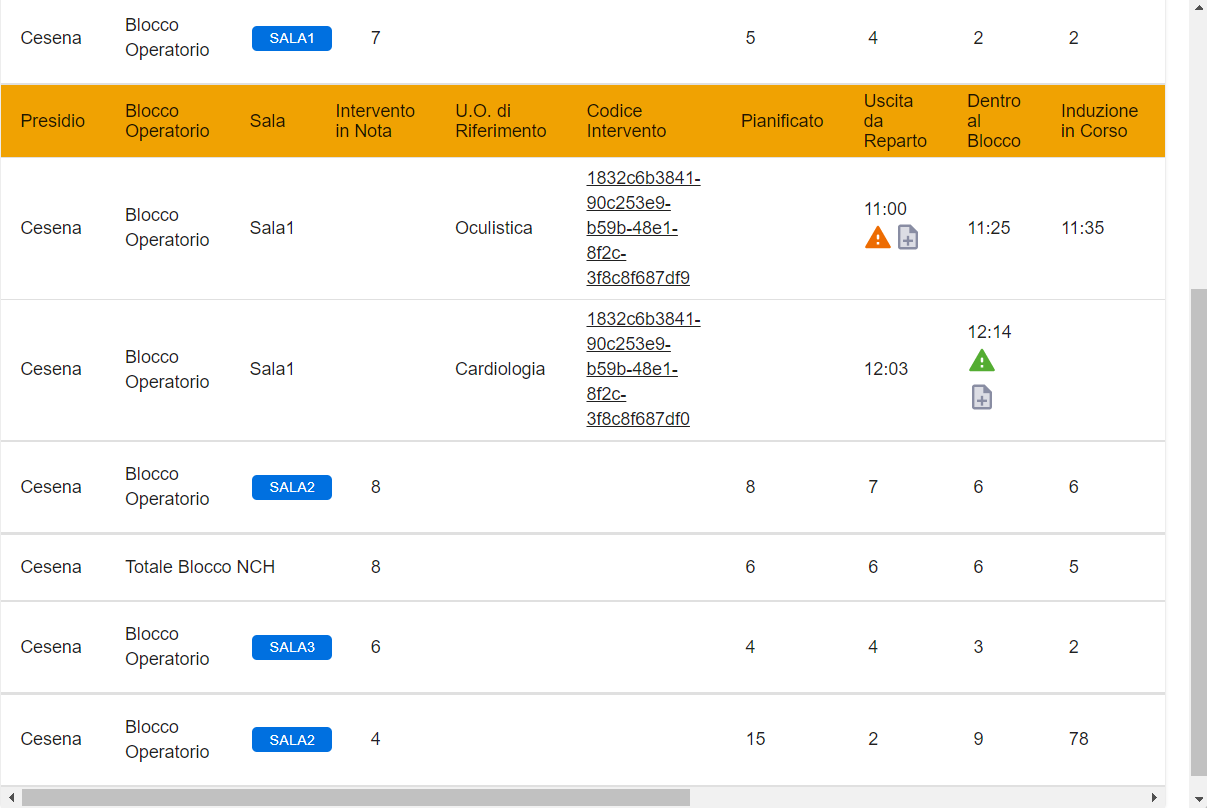
\includegraphics[width=0.9\textwidth]{figures/orm/interventi.png}
     \caption{The expanded view of an operating room, showing the surgical procedures of that room and their steps.}
    \label{fig:orm:surgical_procedures_dashboard}
\end{figure}


This preliminary implementation demonstrates how a \ac{DTE} can be used to support the design of quality-of-life tools and improve the management of complex healthcare processes such as ORM.
%
The current implementation is simplistic and limited in scope, but it provides a demonstrator of applicability of the \ac{DT} paradigm to the domain of ORM, showcasing the potential benefits of the proposed approach including data standardization, legacy system integration, real-time monitoring, anomaly detection, and accountability.

Simulation of the surgical process has been explored to test the proposed \ac{DTE} in a controlled environment.
%
Specifically, as shown in \Cref{fig:orm:anylogic} and \Cref{fig:orm:anylogic2}, an agent-based simulation developed in AnyLogic\footnote{\url{https://www.anylogic.com/}} has been used to model the patient flow through the operating rooms and generate synthetic data that can feed a prototype implementation of the \ac{DTE}.

The simulation models the process assuming a hospital with 3 operating rooms, and a variable number of medical professionals currently on shift. 
%
Patients are scheduled for surgery according to a predefined plan, but random events can occur that may lead to delays in the process.
%
The simulation allows for key event in the patient flow to be tracked, generating traces of events that can be used to communicate with the relevant \acp{DT} in the \ac{DTE} prototype.


\begin{figure}[ht]
    \centering
    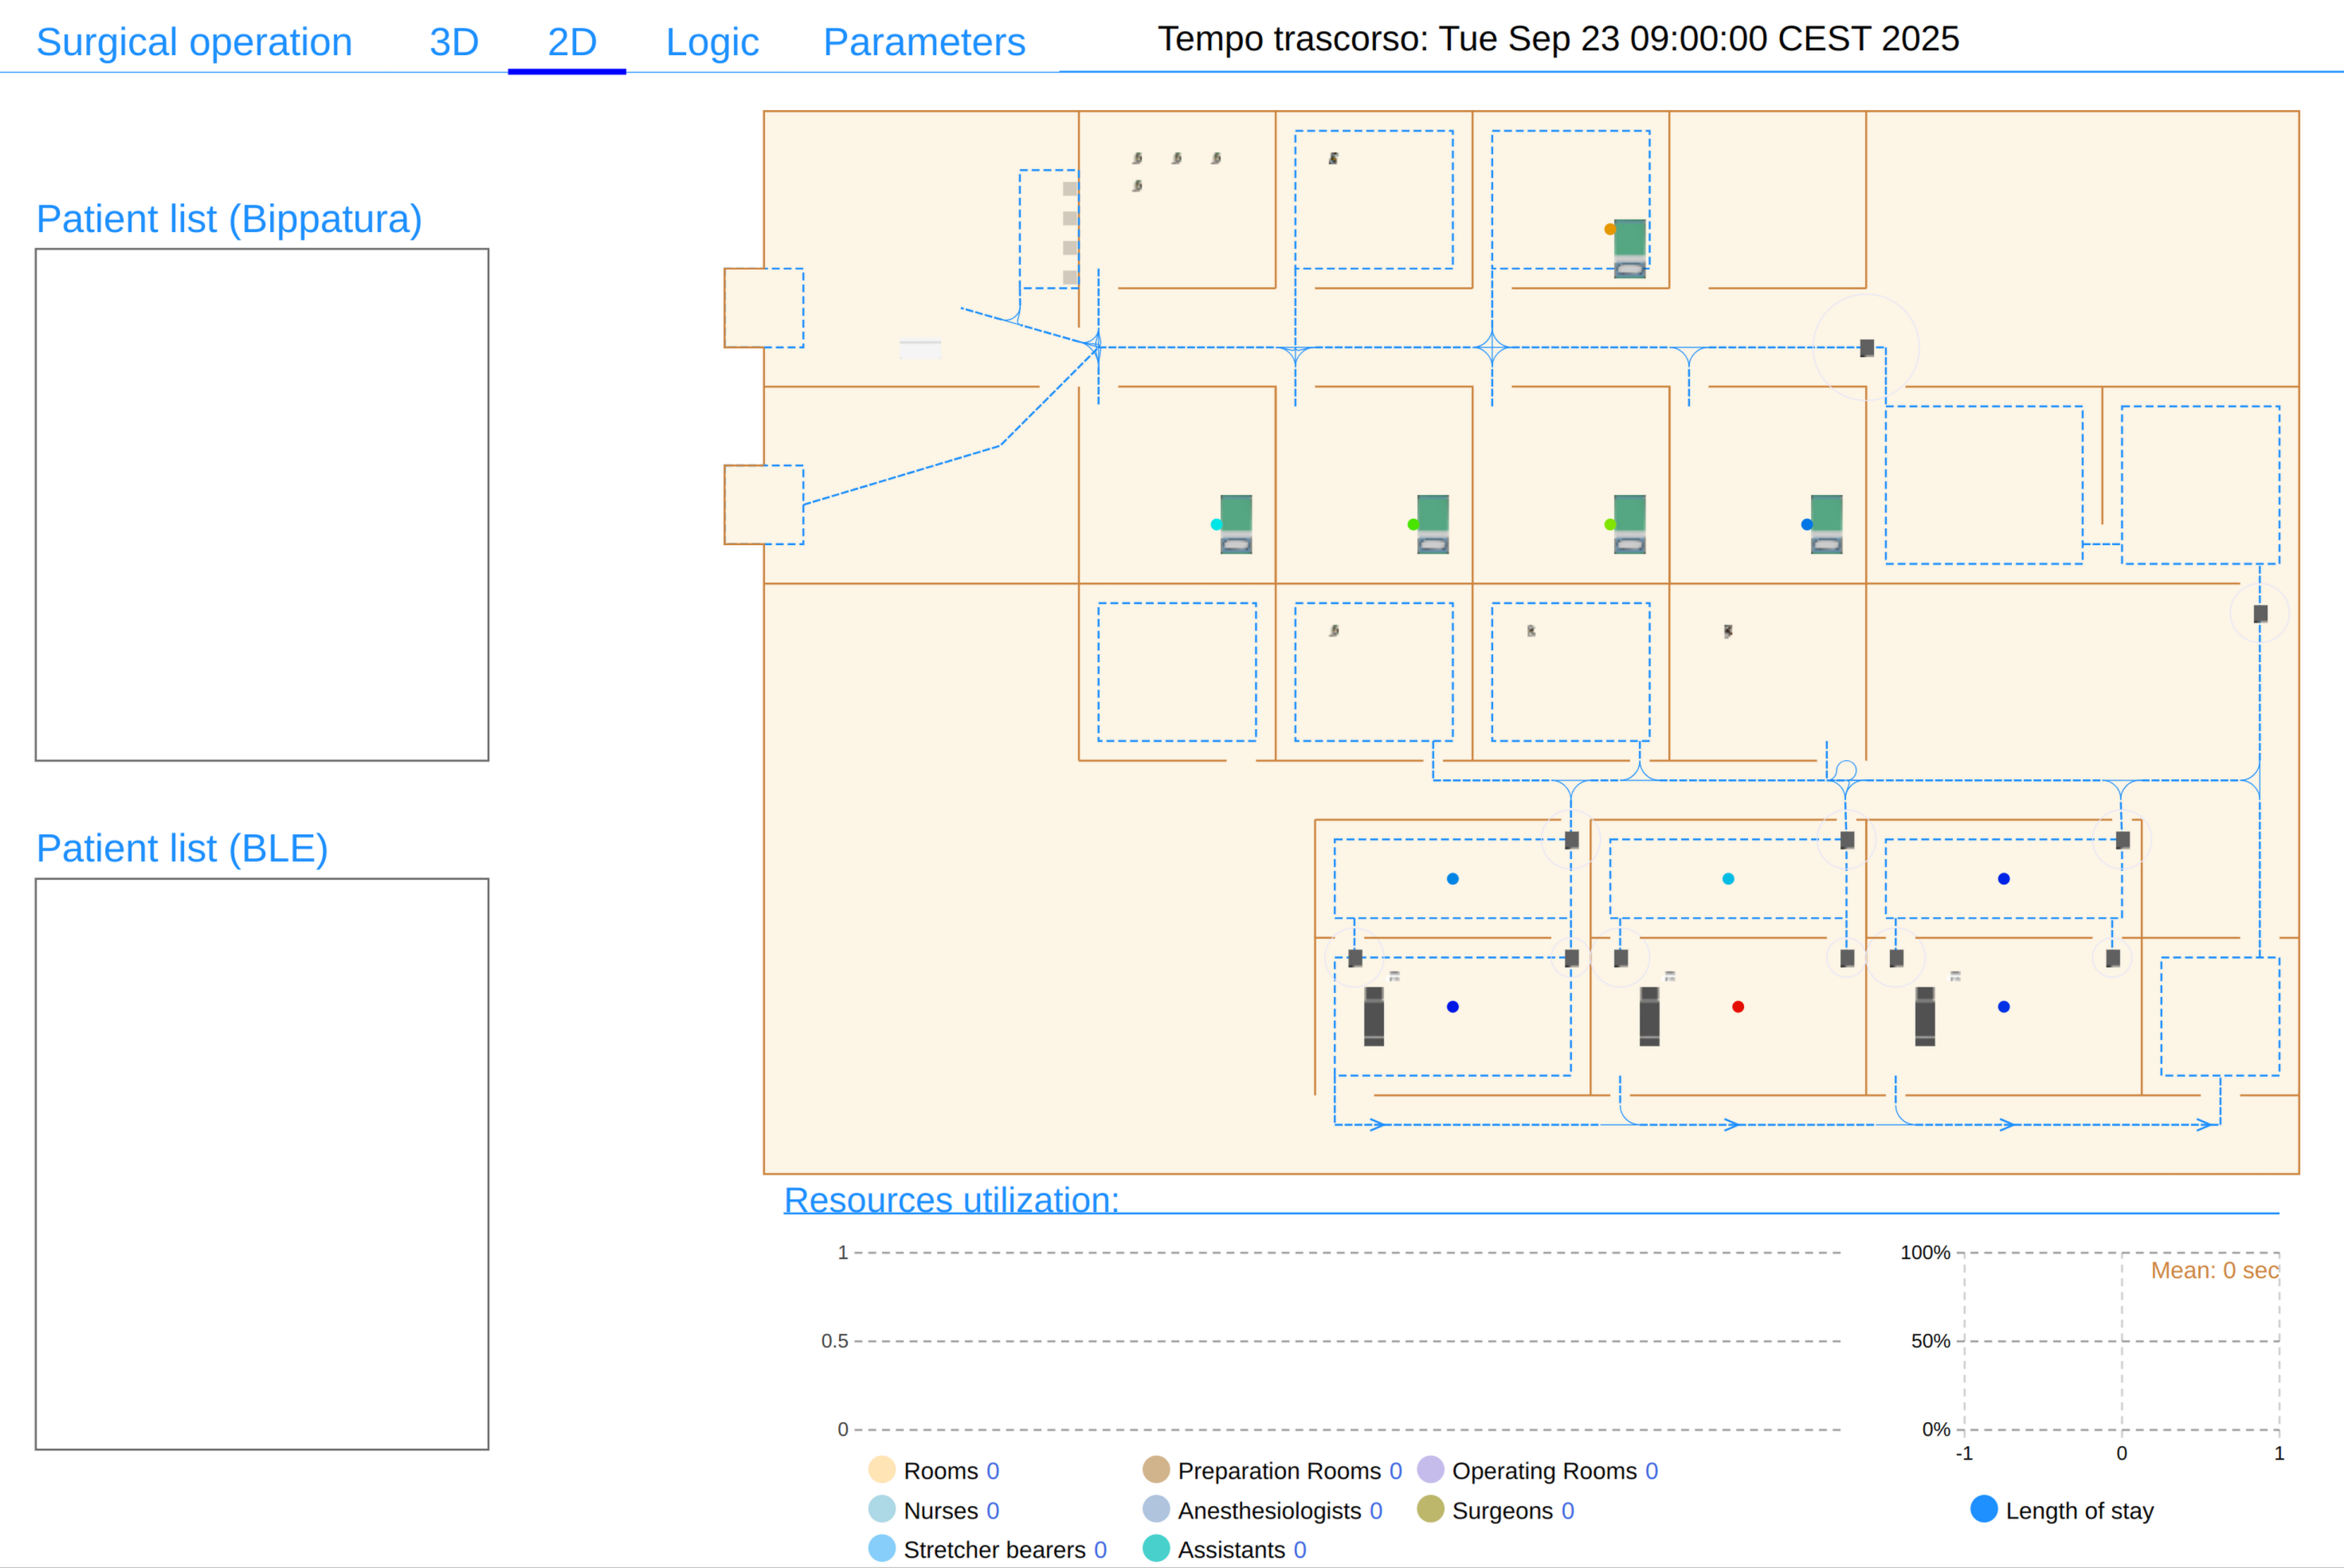
\includegraphics[width=0.7\textwidth]{figures/orm/anylogic.png}
    \caption{Snapshot of the 2D view of the AnyLogic simulation of surgical processes used to generate synthetic data for the DTE prototype.}
    \label{fig:orm:anylogic}
\end{figure}

\begin{figure}[ht]
    \centering
    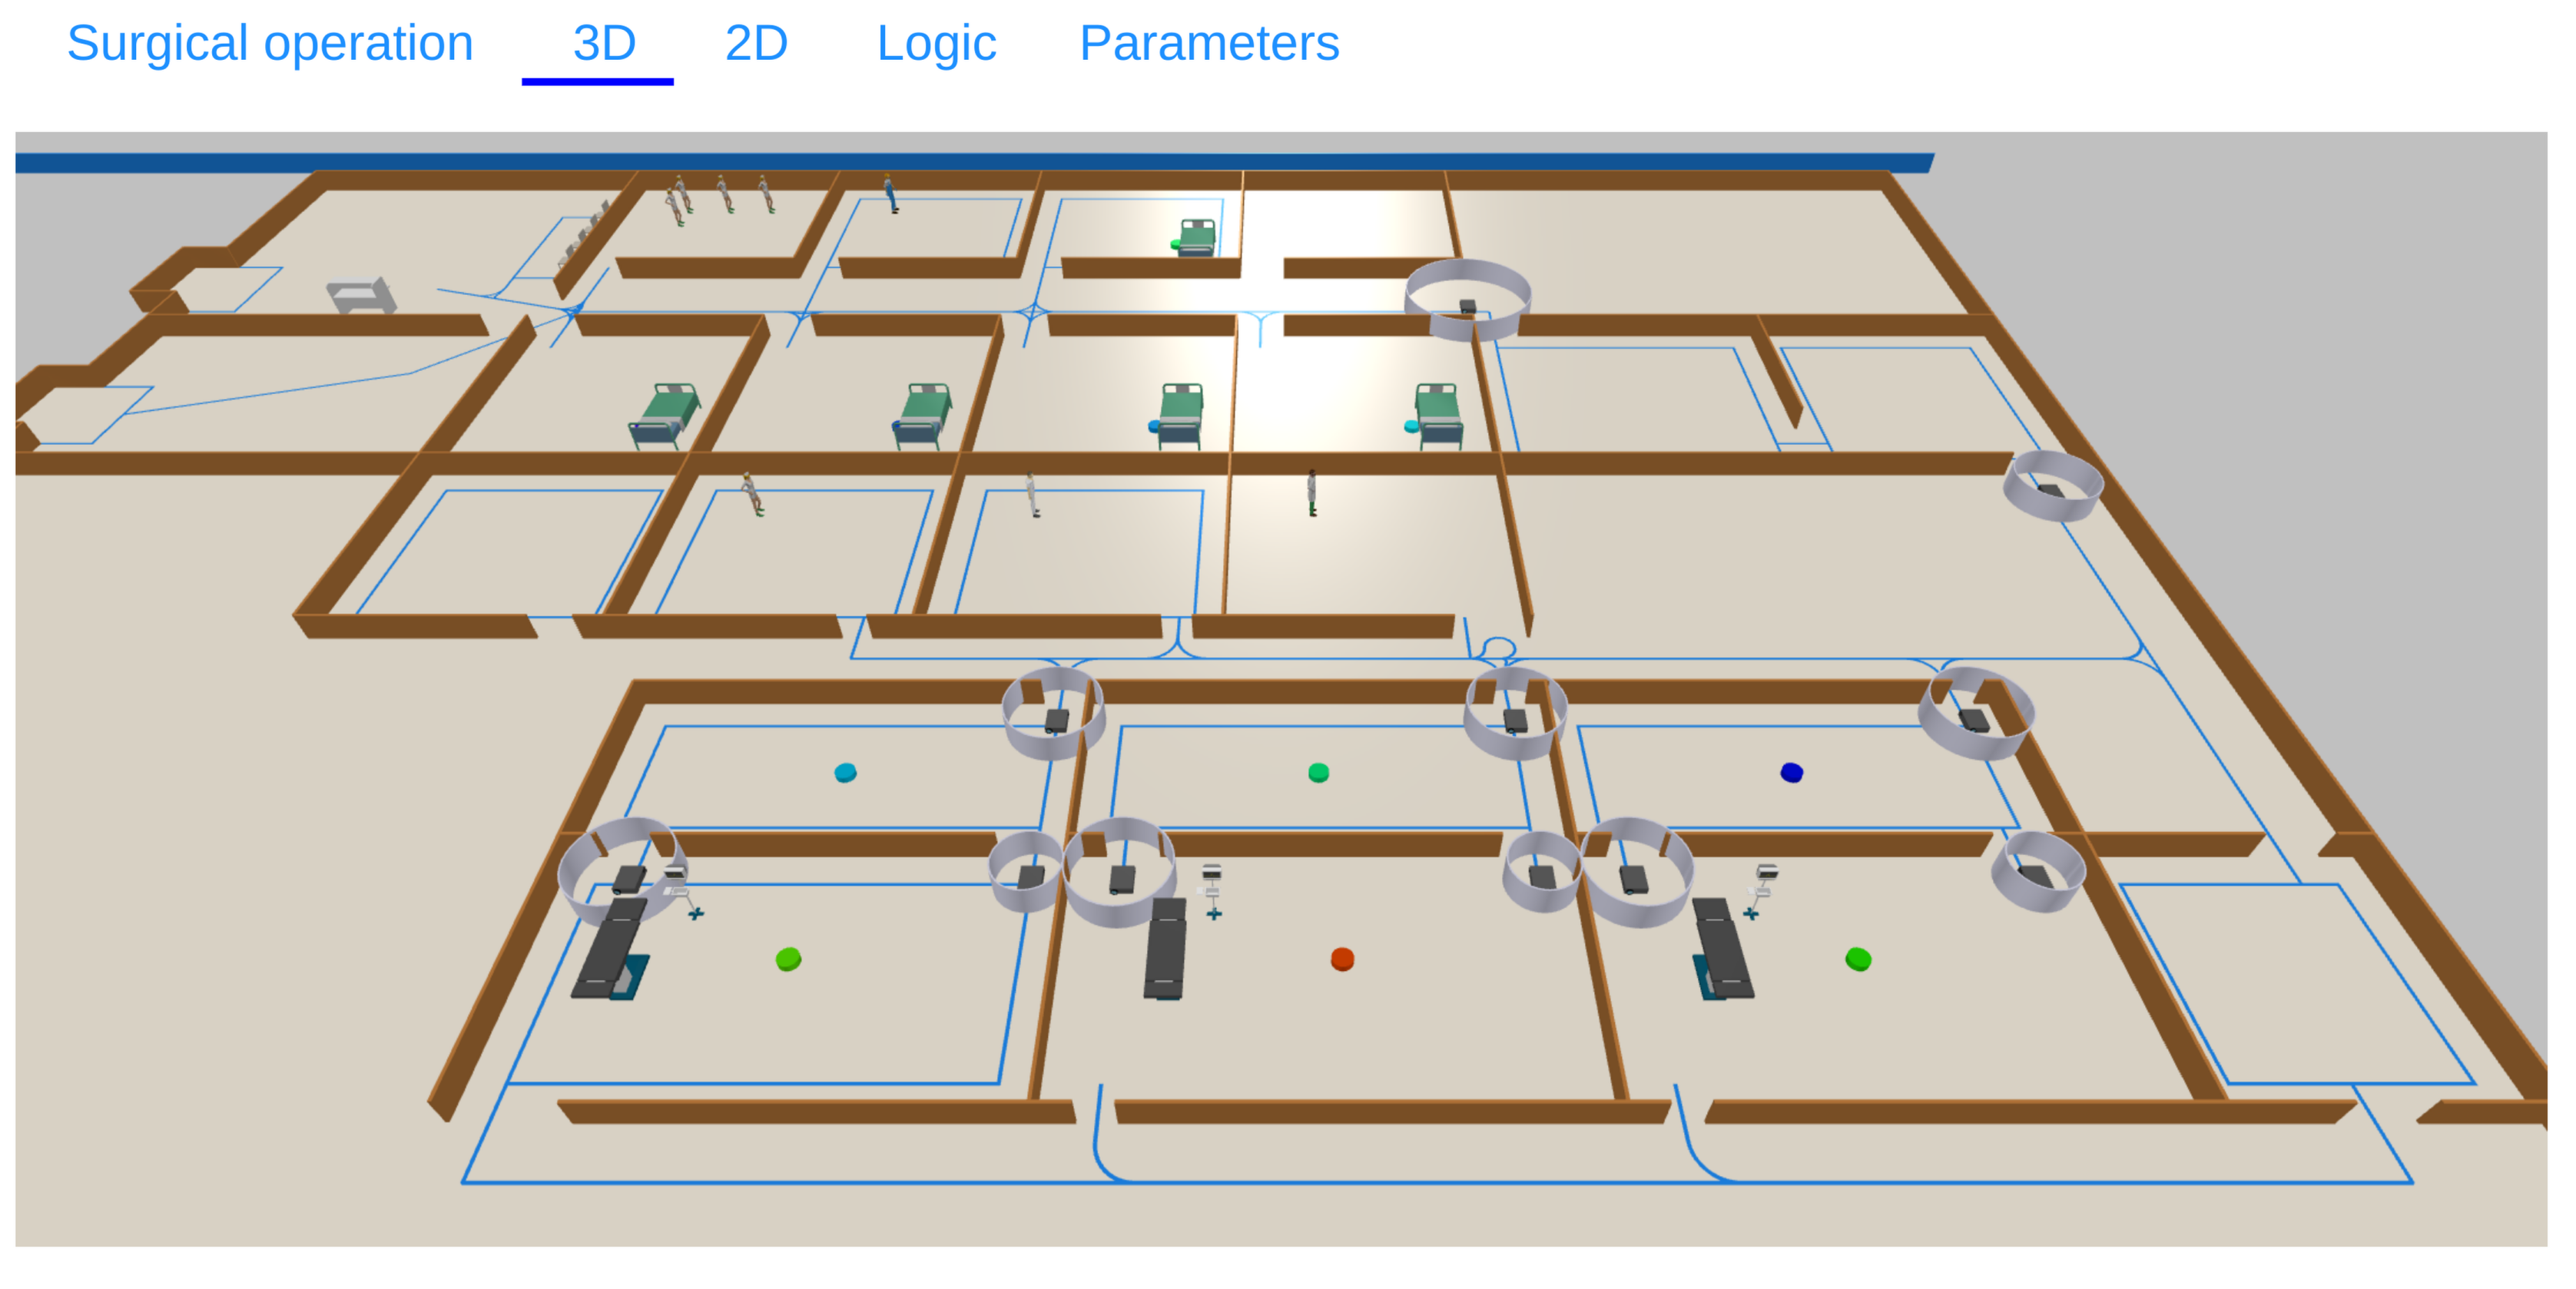
\includegraphics[width=0.9\textwidth]{figures/orm/anylogic2.png}
    \caption{Snapshot of the 3D view of the AnyLogic simulation of surgical processes used to generate synthetic data for the DTE prototype.}
    \label{fig:orm:anylogic2}
\end{figure}

Although in this preliminary implementation the focus has been on using the simulation as a tool to support development of the \ac{DTE} prototype, in future works the simulation model could be integrated into the \ac{DTE} itself to enhance the capabilities of the system in terms of predictive analytics and scenario evaluation.

